\documentclass{IEEEcsmag}

\usepackage[colorlinks,urlcolor=blue,linkcolor=blue,citecolor=blue]{hyperref}

\usepackage{upmath}

\jvol{XX}
\jnum{XX}
\paper{8}
\jmonth{May/June}
\jname{Computing in Science and Engineering}
\pubyear{2021}
\newtheorem{theorem}{Theorem}
\newtheorem{lemma}{Lemma}

\setcounter{secnumdepth}{0}

\begin{document}

\sptitle{Department: Head}
\editor{Editor: Name, xxxx@email}

\title{PyExaFMM: Designing a highly-performant particle fast multipole solver in Python with Numba}

\author{\ S. Kailasa}
\affil{\ Department of Mathematics, University College London}

\author{\ T. Betcke}
\affil{\ Department of Mathematics, University College London}

\author{\ T. Wang}
\affil{\ Department of Mechanical and Aerospace Engineering, The George Washington University}

\author{\ L. A. Barba}
\affil{\ Department of Mechanical and Aerospace Engineering, The George Washington University}

\markboth{Department Head}{Paper title}

\begin{abstract}
PyExaFMM is a Python based kernel-independent particle fast multipole method implementation, built on the success of the ExaFMM project, to answer the question of whether we could develop a highly-performant scientific code without resorting to a lower level language. The FMM is a good case study for understanding the maturity of Python for developing high-performance software, due its reliance on a complex heirarchical octree data structure. In this article we explore the software engineering and mathematical techniques used to extract performance for PyExaFMM, and we report that we are able to achieve runtimes within $\mathcal{O}(10)$ of the state of the art C++ implementation, with comparable accuracy for three dimensional electrostatic problems.

\end{abstract}

\maketitle

\chapterinitial{The Fast Multipole Method} [FMM], originally developed by Greengard and Rokhlin \cite{Greengard1987}, approximates the solution of the so called $N$ body problem, in which one seeks to calculate the pairwise interactions between $N$ objects. This problem arises in numerous contexts in science and engineering, for example in the calculation of the resulting electrostatic potentials due to a set of charged particles. Considering the calculation of electrostatic potential as our model problem, the potential, $\phi(x_j)$, for a given charged particle at position $x_j$, or `target', due to $N$ particles at positions $x_i$, or `sources', where $i \in [1, ..., N]$, each with a charge $q_i$, can be written as,

\begin{eqnarray}
	\phi(x_j) = \sum_{i=1}^{N} K(x_i, x_j) q_i,
\label{eq:sec:intro:nbody_problem}
\end{eqnarray}

here $K(\cdot, \cdot)$ is called the Green's function, or kernel function, which for electrostatic problems in three dimensions is,

\begin{eqnarray}
	K(x, y) = \frac{1}{4\epsilon_0\pi|x-y|},
\label{eq:sec:intro:laplace_kernel}
\end{eqnarray}

where $\epsilon_0$ is the permittivity of free space. This kernel function is often referred to as the Laplace kernel.

[ Find more scientific examples where the algorithm is useful for better context ]

Attempting to evaluate the sum in (\ref{eq:sec:intro:nbody_problem}) directly for $N$ target particles at positions $x_j$ where $j \in [1,...,N]$ due to $N$ sources, results in algorithm of $\mathcal{O}(N^2)$ runtime complexity, however the FMM is able to approximate (\ref{eq:sec:intro:nbody_problem}) with just $\mathcal{O}(N)$ runtime complexity, with proscribed error bounds.

The key idea behind the FMM is to encode the potential in the far field due to a cluster of particles with a representative analytic \textit{multipole expansion} centered on the cluster, which can be truncated to tune for desired accuracy. This truncation allows one to approximate the sum in (\ref{eq:sec:intro:nbody_problem}) with fewer calculations. In regions centered far away from the cluster, their potentials can be encoded in a \textit{local expansion}. Translations between multipole and local expansions can be done analytically, and are critical in the development of the $\mathcal{O}(N)$ algorithm.

In the FMM, the problem domain is described by a box enclosing all targets and sources, which is hierarchically partitioned into a structure known as a quadtree in two dimensions, and an octree in three dimensions. The partioning is done recursively, such that at the first level of refinement the box is partitioned into four equal sized parts in two dimensions (or eight in three dimensions), known as it's children, which are each subsequently refined in a similar fashion. The level of refinement is defined by a parameter dictating the maximum allowable number of particles contained within a box. The finest boxes covering a portion of the domain that remain after refinement are known as leaves. One can choose to refine \textit{adaptively}, such that the leaves may be of different sizes, reflective of the underlying particle distribution, or \textit{non-adaptively}, such that the leaves are all of a uniform size.

The FMM then consists of two sequential traversals through this tree, where boxes are considered level by level, with level zero being the unrefined box which defines the domain, level one being the level of its child boxes, and so forth. Firstly, during the \textit{upward pass}, multipole expansions for particles contained in boxes at the highest level of refinement, or leaf level, of the tree are formed. This is referred to as the \textit{particle-to-multipole} [P2M] step. In order to obtain the multipole expansion at their parent level, the multipole expansions of a given box's children at the leaf level have their expansion centre translated to the centre of their shared parent box, and the coefficients are summed. This is referred to as the \textit{multipole-to-multipole} [M2M] step. This is repeated bottom-up, level by level, until one is left with the multipole expansions of all boxes in the tree.

Subsequently, during the \textit{downward pass}, the multipole expansions of non-adjacent boxes of a given box are defined as being in its far-field. In order to evaluate their contribution towards the potential for particles within a given box, one translates their multipole expansion to a local expansion centered at the given box. This is referred to as the \textit{multipole-to-local} [M2L] step. The local expansion is then transferred to the children of the given box by shifting the expansion centre. Proceeding top-down, considering boxes level by level, one is left with the local expansions for each leaf box. This is referred to as the \textit{local-to-local} [L2L] step. Crucially the extent of the far field not already encapsulated in the local expansion shrinks as we descend down the octree. This is because the far field of a box's parent is already captured in the child's local expansion. These local expansions compress all of the contribution from the far field towards the potential for targets within a given leaf. Therefore the far-field's effect on the potential of targets within a leaf box is entirely described by the local expansion. The evaluation of the local expansion at the target points in a given leaf box is known as the \textit{local-to-particle} [L2P] step. Finally, the near fields of a given leaf box are  evaluated directly using (\ref{eq:sec:intro:nbody_problem}), this is referred to as the \textit{particle-to-particle} [P2P] step. As there are a fixed number of particles per leaf node, the complexity of this direct near field evaluation is bounded. This scheme is illustrated for a two dimensional problem, with a uniform quadtree, in figure (\ref{fig:tree_traversal}).

The $\mathcal{O}(N)$ algorithmic runtime complexity can be roughly seen to be the result of the ability to exactly translate between the multipole and local expansions for all boxes deemed to be in the far field, as well as the recursive procedure of the FMM. As a result of this, each box must only consider it's interaction with a constant number of other boxes. As there are $\mathcal{O}(N)$ boxes in a given tree, the entire algorithm can be seen to be bounded by a runtime complexity of $\mathcal{O}(N)$.

The coefficients of a given multipole expansion are kernel-dependent in the sense that they will depend on the form of (\ref{eq:sec:intro:laplace_kernel}), software implementations have to be rewritten for each specific physical model. Fast multipole methods for general kernels \cite{Gimbutas2003} have been developed, however there are fewer methods that rely only on numerical kernel evaluations, rather than analytic series expansions, examples include \cite{Fong2009, Ying2004,Martinsson2007}. The latter approaches are often referred to as kernel-independent fast multipole methods [KIFMM]. PyExaFMM utilizes the approach first presented by Ying et. al \cite{Ying2004}. This KIFMM represents the multipole expansions due to a cluster of charges as set of equivalent densities supported on a surface enclosing the cluster, with the fields generated by the charges matched with the equivalent field via a least-squares fitting in the far field. As originally developed in \cite{Ying2004}, this method generalizes the FMM to non-oscillatory second-order elliptic partial differential equations with constant coefficients, for example the Laplace or Stokes equations. Further work has extended the method to include oscillatory problems \cite{Engquist2007}. Alternatively, Fong et. al \cite{Fong2009} use a Chebyshev based interpolation scheme to approximate the action of the kernel function in the far-field.

At present, numerous high-quality open source implementations exist to solve FMM problems, both using analytic expansions for various kernels \cite{Gimbutas2010}, \cite{Yokota2017}, as well as using the KIFMM of Fong et. al \cite{Bramas2020}, \cite{Agullo2014}, \cite{Agullo2016}, and Ying et. al \cite{Wang2021}, \cite{Lashuk2012}. Many of these implementations are able to scale on supercomputing clusters, and solve problems involving millions of degrees of freedom. Others are designed to be run on a single workstation \cite{Bramas2020, Agullo2014, Wang2021}. These softwares are often developed in compiled languages, such as Fortran or C++, often making use of numerous non-standard libraries and features. On the other hand, many domain specialists usually have limited computational skill-sets, often restricted to subsets of Python for data-analysis or numerical computing, or Matlab. Therefore it is not feasible for many users of to contribute to, or extend, many of these existing libraries without a significant investment in acquiring new computational skills. This problem is not unique to FMM implementations, but is general across high-performance computing [HPC] software.
In recent years high-performance libraries that aid in bypassing the limitations of the Python interpreter have emerged to make it a serious contender for use in developing software for high-performance computing [HPC]. The most interesting example is Numba, a `just in time' compiler for Python. (Some exposition on Numba here, and what it allows us to do HERE) \cite{Lam2015}. Furthermore, the build infrastructure provided by Conda [CITATION FOR CONDA] makes it trivial to develop Python applications for different platforms.

Therefore, the question naturally arises of whether it is feasible to develop a HPC library entirely within Python. The envisioned goal being that of a domain specialist being able to trivially iterate from a Python prototype, to a performant HPC application. An FMM implementation is an excellent case study to understand the maturity of Python for HPC development. As Numba is built to optimize operations on arrays, it represents a challenge to develop efficient representations and operations for the tree on which the algorithm is based. In developing PyExaFMM we aimed to demonstrate the possibility of building an HPC application purely in Python, while achieving comparable performance with state of the art compiled language implementations. This would represent a compromise between usability, and performance, allowing domain specialists to easily contribute to and extend an efficient HPC library.

In this article we begin by providing an overview of the mathematical formulation behind the KIFMM in \cite{Ying2004}, before introducing Numba and discussing how it is used by PyExaFMM to accelerate computations, as well as program efficient data structures. We continue by discussing the mathematical and software based optimizations used by PyExaFMM for performance, and provide an overview of the software design used in order to implement optimizations effectively. We conclude with a discussion comparing the performance, in terms of accuracy, runtimes, and memory footprint, with the comparable state-of-the-art C++ implementation from the ExaFMM project, ExaFMM-T \cite{Wang2021}.

\section{THE KERNEL-INDEPENDENT FAST MULTIPOLE METHOD}

In this article we begin by providing an overview of the mathematical formulation behind the KIFMM in \cite{Ying2004}, before introducing Numba and discussing how it is used by PyExaFMM to accelerate computations, as well as program efficient data structures. We continue by discussing the mathematical and software based optimizations used by PyExaFMM for performance, and provide an overview of the software design used in order to implement optimizations effectively. We conclude with a discussion comparing the performance, in terms of accuracy, runtimes, and memory footprint, with the comparable state-of-the-art C++ implementation from the ExaFMM project, ExaFMM-T \cite{Wang2021}.


\subsection{Algorithm}

\section{TECHNIQUES FOR ACHIEVING PERFORMANCE}

\subsection{What is Numba?}

What is does, how is it useful? Where do we use it, and why there. How much difference can it make in an idealized routine. What doesn't work, why doesn't it work. Where to be careful. Programming to an (invisible) framework \dots

Where is numba used heavily? Tree construction routines on Morton coordinates. Multithreading of tree construction, as well as P2M evaluation. Experiment to demonstrate the speed of kernel evaluation, with caveat that data must be pre-organised.

\subsection{Precomputing Operators}

Transfer vectors, hashing, HDF5, loading into memory.

\subsection{Compressing the M2L step with a randomised SVD}

Introduce \cite{Ying2004}. Numerical bounds on error out of scope, but show how experiments demonstrate that the FMM error dominates the SVD error.

\subsection{Software Architecture}

The key is separating routines to be accelerated, and organising data ready to run. The data organisation part (and it's slowness) should be demonstrated as a bottleneck using experiment.

\section{PERFORMANCE COMPARISON WITH STATE OF THE ART}

Description of main experiments, and how they are conducted. What are the main results? Are they expected from theory? What conclusions can be drawn about developing HPC codes entirely in Python, is it worth it?

% \begin{figure}
% \centerline{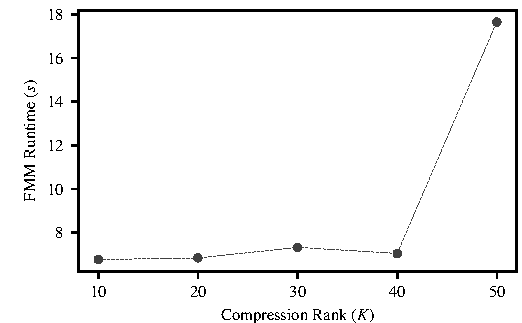
\includegraphics[width=18.5pc]{figures/compression_runtime.pdf}}
% \caption{Compression Rank and runtime}
% \end{figure}

% \begin{figure}
% \centerline{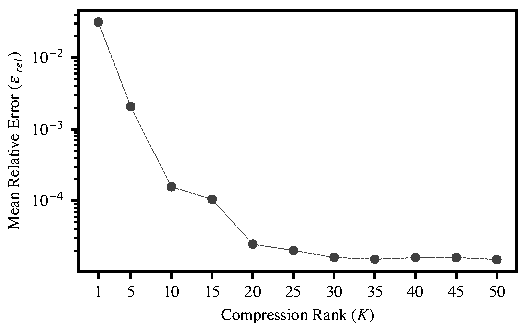
\includegraphics[width=18.5pc]{figures/compression_accuracy.pdf}}
% \caption{Compression Rank and accuracy}
% \end{figure}

% \begin{figure}
% 	\centerline{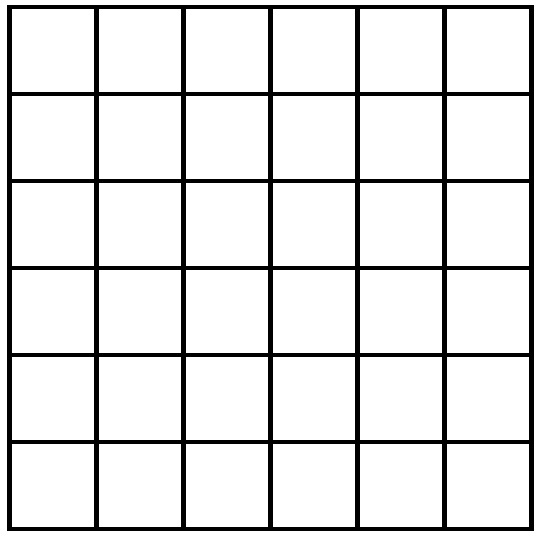
\includegraphics[width=18.5pc]{figures/interaction_lists.pdf}}
% 	\caption{Compression Rank and accuracy}
% \end{figure}

% Larger figure
\begin{figure*}
\centerline{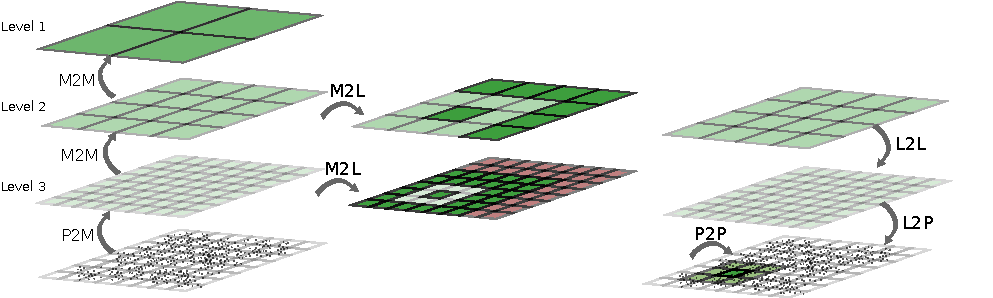
\includegraphics {figures/algorithm.pdf}}
\caption{FMM illustrated for a two dimensional problem.}
\label{fig:tree_traversal}
\end{figure*}

% \begin{figure*}
% \centerline{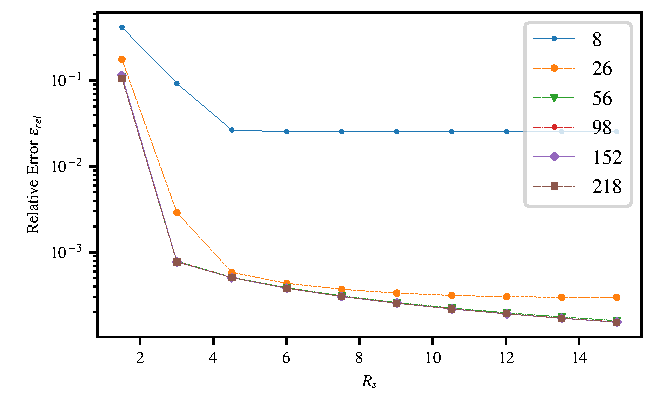
\includegraphics[width=26pc]{figures/pyexafmm_multipole_convergence.pdf}}
% \caption{PyExaFMM Multipole Expansion Convergence}
% \end{figure*}

% \begin{figure*}
% \centerline{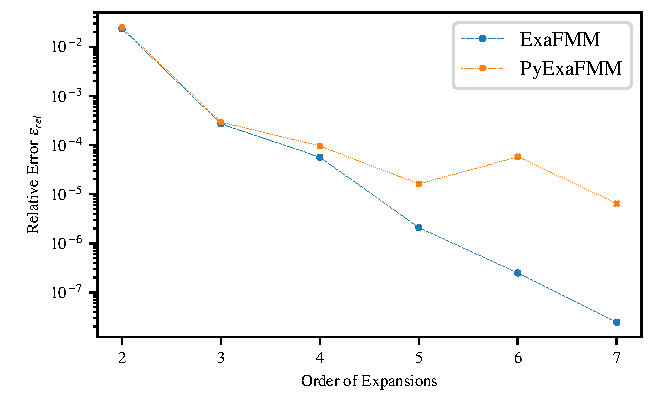
\includegraphics[width=26pc]{figures/potential_convergence.pdf}}
% \caption{Potential Convergence Comparison}
% \end{figure*}


% \begin{table}
% \caption{Units for magnetic properties.}
% \label{table}
% \small
% \begin{tabular*}{17.5pc}{@{}|p{29pt}|p{63pt}<{\raggedright}|p{80pt}<{\raggedright}|@{}}
% \hline
% Symbol&
% Quantity&
% Conversion from Gaussian and  CGS EMU to SI$^{\mathrm{a}}$ \\
% \hline
% $\Phi $&
% Magnetic flux&
% 1 Mx $\to  10^{-8}$ Wb $= 10^{-8}$ V $\cdot$ s \\
% $B$&
% Magnetic flux density,   magnetic induction&
% 1 G $\to  10^{-4}$ T $= 10^{-4}$ Wb/m$^{2}$ \\
% $H$&
% Magnetic field strength&
% 1 Oe $\to  10^{-3}/(4\pi )$ A/m \\
% $m$&
% Magnetic moment&
% 1 erg/G $=$ 1 emu   $\to 10^{-3}$ A $\cdot$ m$^{2} = 10^{-3}$ J/T \\
% $M$&
% Magnetization&
% 1 erg/(G $\cdot$ cm$^{3}) =$ 1 emu/cm$^{3}$   $\to 10^{-3}$ A/m \\
% 4$\pi M$&
% Magnetization&
% 1 G $\to  10^{-3}/(4\pi )$ A/m \\
% $\sigma $&
% Specific magnetization&
% 1 erg/(G $\cdot$ g) $=$ 1 emu/g $\to $ 1 A $\cdot$ m$^{2}$/kg \\
% $j$&
% Magnetic dipole   moment&
% 1 erg/G $=$ 1 emu   $\to 4\pi \times  10^{-10}$ Wb $\cdot$ m \\
% $J$&
% Magnetic polarization&
% 1 erg/(G $\cdot$ cm$^{3}) =$ 1 emu/cm$^{3}$  $\to 4\pi \times  10^{-4}$ T \\
% $\chi , \kappa $&
% Susceptibility&
% 1 $\to  4\pi $ \\
% $\chi_{\rho }$&
% Mass susceptibility&
% 1 cm$^{3}$/g $\to  4\pi \times  10^{-3}$ m$^{3}$/kg \\
% $\mu $&
% Permeability&
% 1 $\to  4\pi \times  10^{-7}$ H/m   $= 4\pi \times  10^{-7}$ Wb/(A $\cdot$ m) \\
% $\mu_{r}$&
% Relative permeability&
% $\mu \to \mu_{r}$ \\
% $w, W$&
% Energy density&
% 1 erg/cm$^{3} \to  10^{-1}$ J/m$^{3}$ \\
% $N, D$&
% Demagnetizing factor&
% 1 $\to  1/(4\pi )$ \\
% \hline
% \multicolumn{3}{@{}p{17.5pc}@{}}{Vertical lines are optional in tables. Statements that serve as captions for
% the entire table do not need footnote letters. }\\
% \multicolumn{3}{@{}p{17.5pc}@{}}{$^{\mathrm{a}}$Gaussian units are the same as cg emu for magnetostatics; Mx
% $=$ maxwell, G $=$ gauss, Oe $=$ oersted; Wb $=$ weber, V $=$ volt, s $=$
% second, T $=$ tesla, m $=$ meter, A $=$ ampere, J $=$ joule, kg $=$
% kilogram, H $=$ henry.}
% \end{tabular*}
% \label{tab1}
% \end{table}


\section{CONCLUSION}

What have we learned, what will we be working on next?

\section{ACKNOWLEDGMENT}

SK is supported by EPSRC Studentship 2417009.

\bibliography{pyexafmm}
\bibliographystyle{ieeetr}

\begin{IEEEbiography}{Srinath Kailasa}{\,} is a graduate student at University College London. He is currently pursuing a PhD in Computational Mathematics, having received an MPhys in Physics (2017) and an MSc Scientific Computing (2020) from the University of Durham, and University College London respectively. His research interests are in high-performance and scientific computing. Contact him at srinath.kailasa.18@ucl.ac.uk.
\end{IEEEbiography}

\begin{IEEEbiography}{Timo Betcke}{\,}is a Professor of Computational Mathematics at University College London. Contact him at t.betcke@ucl.ac.uk.
\end{IEEEbiography}

\begin{IEEEbiography}{Tingyu Wang}{\,}is a PhD student in Mechanical Engineering at the George Washington University. Contact him at twang66@email.gwu.edu.
\end{IEEEbiography}

\begin{IEEEbiography}{Lorena. A. Barba}{\,}is a Professor of Mechanical and Aerospace Engineering at the George Washington University.  Contact her at labarba@email.gwu.edu.
\end{IEEEbiography}

\end{document}

